%!TEX root = ../physical-olympics-2.tex
\chapter{物理光学}


\section{经典色散理论}

蓝天,\,白云,\,红太阳.\,在简单的自然现象中蕴含着光在传播过程中的另外一种典型的现象:\,\emph{散射}(scattering).\,而散射却又是一个多么复杂的现象!\,要完全理解散射,\,我们得研究光的吸收与发射,\,因为光与物质中分子的相互作用其实本质上可以看成吸收与发射,\,这是\emph{分子光学}(molecular optics)的研究范畴.\,其次,\,光在介质中的衰减(吸收),\,不同颜色的光折射率的不同(色散)其实都导致了一类散射现象(瑞利散射).\,但是还有不同的散射现象则表现出不用的特性,\,需要从更宏观或更微观的角度去建立新的理论来解释他们.

不同于以往在透明介质中的平面波传播,\,新的现象需要新的平面波模型.

\subsection{复波矢与复折射率}

我们在波动方程的解中引入复数是为了更好地描述振动形式的解.\,但这却忽视了另一种解的存在性.\,就是如果波矢$\bs{k}$本身亦为复数,\,由于同时又是一个矢量,\,可以表示为$\bs{k}=\bs{\alpha}+\ui\bs{\beta}$.\,代入场的空间部分:
\[A(\bs{r})=A_0\ue^{\ui \bs{k}\cdot \bs{r}}=A_0\ue^{- \bs{\beta}\cdot \bs{r}}\ue^{\ui \bs{\alpha}\cdot \bs{r}}\]

这就代表了一个沿$\bs{\alpha}$方向传播,\,沿$\bs{\beta}$方向衰减的平面波.\,而$\bs{\alpha}$为波矢的实部,\,$\bs{\beta}$为波矢的虚部:
\[\bs{\alpha} =\mathfrak{Re} (\bs{k})\quad;\quad \bs{\beta}=\mathfrak{Im} (\bs{k})\]

这种波可不可以在真空中传播?\,出人意料的是这居然是可能的.\,因为如果代入真空中的亥姆霍兹方程:
\[\nabla ^2 A+\frac{\omega^2}{c^2}A=0\]

便会发现这只需要要求:
\[\bs{k}^2=(\bs{\alpha}+\ui \bs{\beta})\cdot(\bs{\alpha}+\ui \bs{\beta})=\frac{\omega^2}{c^2} \quad \Rightarrow \quad \alpha^2-\beta^2=\frac{\omega^2}{c^2},\,\bs{\alpha}\cdot\bs{\beta}=0\]

\begin{wrapfigure}[12]{o}[0pt]{7cm}
\centering
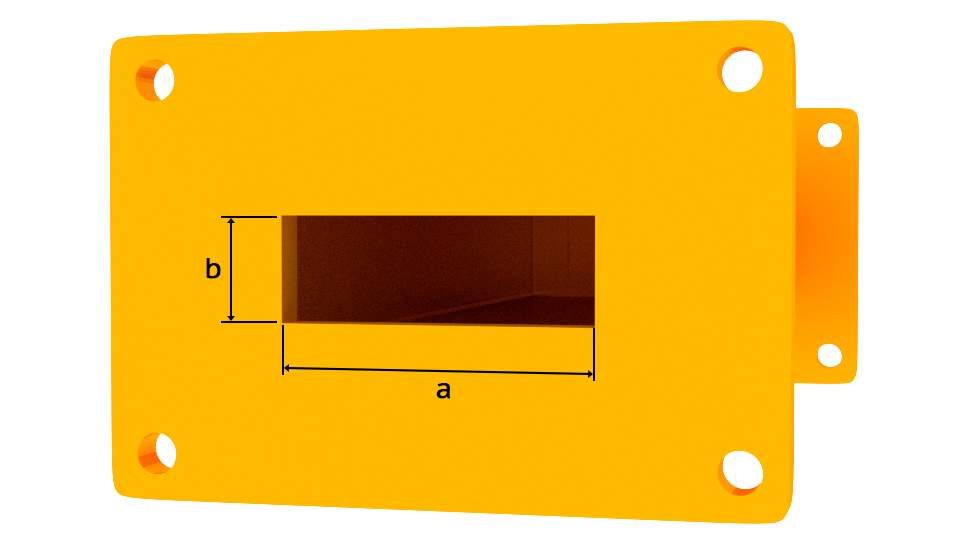
\includegraphics[width=7cm]{image/16-1-1.jpg}
\caption{矩形波导}
\end{wrapfigure}
这样的波我们并不陌生,\,早在几何光学我们介绍光的全反射时便研究过另一侧界面中的隐失波场便是以上形式.\,更典型地,\,在$a\times b$的矩形波导中传播的波满足:
\[(\frac{2\pi}{\lambda_x})^2+(\frac{2\pi}{\lambda_y})^2+(\frac{2\pi}{\lambda_z})^2=\frac{\omega^2}{c^2} \]
\[\lambda_x=\frac{2b}{m},\, \lambda_y=\frac{2a}{n},\,m,\,n=1,\,2\cdots\]

此时在$x,\,y$方向的振动是驻波,\,$z$方向传播的波则是行波.\,$x,\,y$方向要形成驻波是因为在边界的导体上要符合相同的边界条件,\,所以或都是波腹,\,或都是波节.\,亦可以用同一个平面波在侧面上的多次反射的叠加来理解这种兼具驻波和行波特质的场.\,我们发现模式为$(m,\,n)$的波,\,会有一个截止角频率$\omega_c$,\,如果角频率低于此值使得波无法向前传播:
\[\omega_c=c\sqrt{\left(\frac{m\pi}{a}\right)^2+\left(\frac{n\pi}{b}\right)^2}\]

那如果在波导的起点的天线给出信号角频率$\omega<\omega_c$会发生什么情况?\,此时就是$z$方向波矢$k_z$变为虚数,\,意味着波沿$z$方向不是传播而是衰减:
\[\bs{k}=\bs{\alpha}+\ui\bs{\beta}\]
\[\bs{\alpha}=\left( \frac{m\pi}{a},\, \frac{n\pi}{b},\, 0\right)\quad,\quad\bs{\beta}=\left(0 ,\,0 ,\, \sqrt{\left(\frac{m\pi}{a}\right)^2+\left(\frac{n\pi}{b}\right)^2-\frac{\omega^2}{c^2}}\right)\]

在真空中尚可以产生衰减的波\footnote{事实上,\,只需要亚波长的结构便可造成衰减.},\,更何况在各种介质中.\,事实上,\,描述光在介质中随着传播的距离而衰减的现象早有一经验公式,\,即\emph{比尔-朗博-布葛律}(Beer-Lambert-Bouguer law):
\[\frac{I(l)}{I(0)}=\ue^{-\left(\sum_{i} n_i\sigma_i\right) l}\]

其中$I(0)$为在传播$l$前的光强,\,$I(l)$为在传播$l$后的光强.\,$n_i$是构成介质的第$i$种分子的数密度,\,$\sigma_i$为描述其吸收本领的\emph{衰减截面}(attenuation cross section).\,例如对大气来说主要的衰减因素就来自气溶胶,\,干净的海水则能提供200m左右的透光带,\,如果有的话,\,浮游植物含有的光合色素是造成衰减的主要原因.\,而对于强衰减性质的介质,\,我们可以唯象地认为波在介质中的传播为:
\[|A(l)|=|A(0)|\ue^{-\beta l}\quad \Rightarrow\quad I(l)=I(0)\ue^{-2\beta l}\]

这样的选择是有道理的.\,下以导电导致的损耗为例:\,在不漏电介质中,\,麦克斯韦关系本应为:
\[\left\{ \begin{array}{l} 
\nabla\cdot \bs{E}=0 \\[3pt] 
\nabla\times \bs{E}+\dfrac{\partial \bs{H}}{\partial t}=\bs{0} \\[3pt]
\nabla\cdot \bs{H}=0 \\[3pt]
\nabla\times \bs{H}-\varepsilon\mu\dfrac{\partial \bs{E}}{\partial t}=\bs{0} \end{array}\right.\]

这样便有:
\[v=\frac{c}{n}=\frac{1}{\sqrt{\varepsilon \mu}}\quad ,\quad k=\frac{\omega}{v}=\omega\sqrt{\varepsilon \mu}\]

但是,\,如果介质漏电,\,且符合$\bs{J}=\sigma \bs{E}$,\,那么以上方程就改写为:
\[\left\{ \begin{array}{l} 
\nabla\cdot \bs{E}=0 \\[3pt] 
\nabla\times \bs{E}+\dfrac{\partial \bs{H}}{\partial t}=\bs{0} \\[3pt]
\nabla\cdot \bs{H}=0 \\[3pt]
\nabla\times \bs{H}-\varepsilon\mu\dfrac{\partial \bs{E}}{\partial t}=\mu_0 \sigma \bs{E} \end{array}\right.\]

对最后一个式子所引发的不同在光学情况下是很好处理的.\,因为单色光总是具有固定的频率$\omega$,\,那么其实以上式子无非是把$\dfrac{\partial}{\partial t}$变成$-\ui \omega$.\,在磁导率被认为几乎等于真空磁导率的情形下,\,这相当于说:
\[\left\{ \begin{array}{l} 
\nabla\cdot \bs{E}=0 \\ 
\nabla\times \bs{E}-\ui \omega \bs{H}=\bs{0} \\
\nabla\cdot \bs{H}=0 \\
\nabla\times \bs{H}+\ui \omega \varepsilon\mu\bs{E}=\bs{0} \end{array}\right. \qquad \xrightarrow{\varepsilon\rightarrow \varepsilon+\ui \frac{\sigma}{\omega}} \qquad
\left\{ \begin{array}{l} 
\nabla\cdot \bs{E}=0 \\
\nabla\times \bs{E}-\ui \omega \bs{H}=\bs{0}  \\
\nabla\cdot \bs{H}=0 \\
\nabla\times \bs{H}+\ui \omega \varepsilon\mu\bs{E}-\ui\sigma \mu \bs{E}=\bs{0} \end{array}\right.
\]

所以对于漏电介质\footnote{即使不漏电,\,也会由于有损耗而等效于有复电容率.},\,通常会有\emph{复电容率}(complex permittivity)的说法\footnote{对于普通的导体,\,也一样可以讨论复电容率,\,或者更常见地,\,\emph{复电导率}(complex conductivity).\,它不仅包含由于原子实部分极化导致的电容性,\,还要包含由于电子运动惯性导致的电感性.},\,它就是以上把电容率和电导率合并以后的新的复常数,\,用它第四个方程就与真空中的方程没有任何区别了,\,除了系数是一个复数:
\[\varepsilon^\prime =\varepsilon+\ui\frac{\sigma}{\omega}:\quad \nabla\times \bs{H}+\ui \omega \varepsilon^\prime\mu\bs{E}=\bs{0}\]

这样一个方程的解是可以完全照搬之前的解的,\,因为数学上可以证明复数解具有可\emph{解析延拓}(analytic continuation)的特性.\,从而容易发现,\,复波矢就变为:
\[\bs{k}^2=\omega^2\varepsilon^\prime \mu\]

这样就得到:
\[\alpha^2-\beta^2=\omega^2\varepsilon \mu\quad ,\quad 2\bs{\alpha}\cdot\bs{\beta}=2\alpha\beta\cos\theta=\omega\sigma\mu>0\]

此时传播波矢$\bs{\alpha}$与衰减波矢$\bs{\beta}$就不一定要垂直了,\,它们必须夹锐角,\,也就是说,\,如果电磁波在漏电介质或者导体中传播,\,沿传播方向必须要衰减.\,我们最后引入光学中使用最多的\emph{复折射率}(complex refraction index),\,按照原来的看法它意味着$k^2=n^2k_0^2=n^2\dfrac{\omega^2}{c^2}=\dfrac{\omega^2}{v^2}$.\,现在要更小心些,\,因为$\bs{k}=\bs{\alpha}+\ui \bs{\beta}$已经包含两个不贡献的波矢部分.\,故我们先对以下表达式开方:
\[\alpha^2-\beta^2+2\ui \alpha\beta\cos\theta=\omega^2\varepsilon^\prime \mu\]
\[\Rightarrow \quad \sqrt{\alpha^2-\beta^2+2\ui \alpha\beta\cos\theta}=n\frac{\omega}{c}=(n_1+\ui n_2)\frac{\omega}{c}\]

通过以上两式对比,\,我们能得到两个方面.\,第一是复折射率实部$n_1$与虚部$n_2$分别是这样依赖于相对介电常数$\varepsilon_r=\varepsilon/\varepsilon_0$和电导率$\sigma$的:
\[n_1=\sqrt{\varepsilon_r}\cdot \sqrt{\frac{1}{2}\left(1+\frac{\sigma^2}{\omega^2\varepsilon^2}+\sqrt{1+\frac{\sigma^2}{\omega^2\varepsilon^2}}\right)}\]
\[n_2=\frac{\sigma}{\sqrt{\varepsilon_r}\omega\varepsilon_0}\cdot\sqrt{\frac{1}{2}\left(1+\frac{\sigma^2}{\omega^2\varepsilon^2}+\sqrt{1+\frac{\sigma^2}{\omega^2\varepsilon^2}}\right)^{-1}}\]

第二组关系式如果已知了介质的两个折射率,\,那么在介质中传播的波的两个波矢$\alpha$和$\beta$需要满足的关系为:
\[\alpha^2-\beta^2=(n_1^2-n_2^2)\frac{\omega^2}{c^2}\]
\[\alpha\beta\cos\theta=n_1n_2\frac{\omega^2}{c^2}\]

只有当$\theta=0$才恰有:
\[\alpha=n_1\frac{\omega}{c}\quad,\quad\beta=n_2\frac{\omega}{c}\]


\subsection{经典电子论的解释}

下面我们来介绍历史上发挥了重要作用的经典电子论.\,它虽然不够精确但物理图像十分重要.

\begin{wrapfigure}[17]{o}[0pt]{6cm}
\centering
\vspace{-3pt}
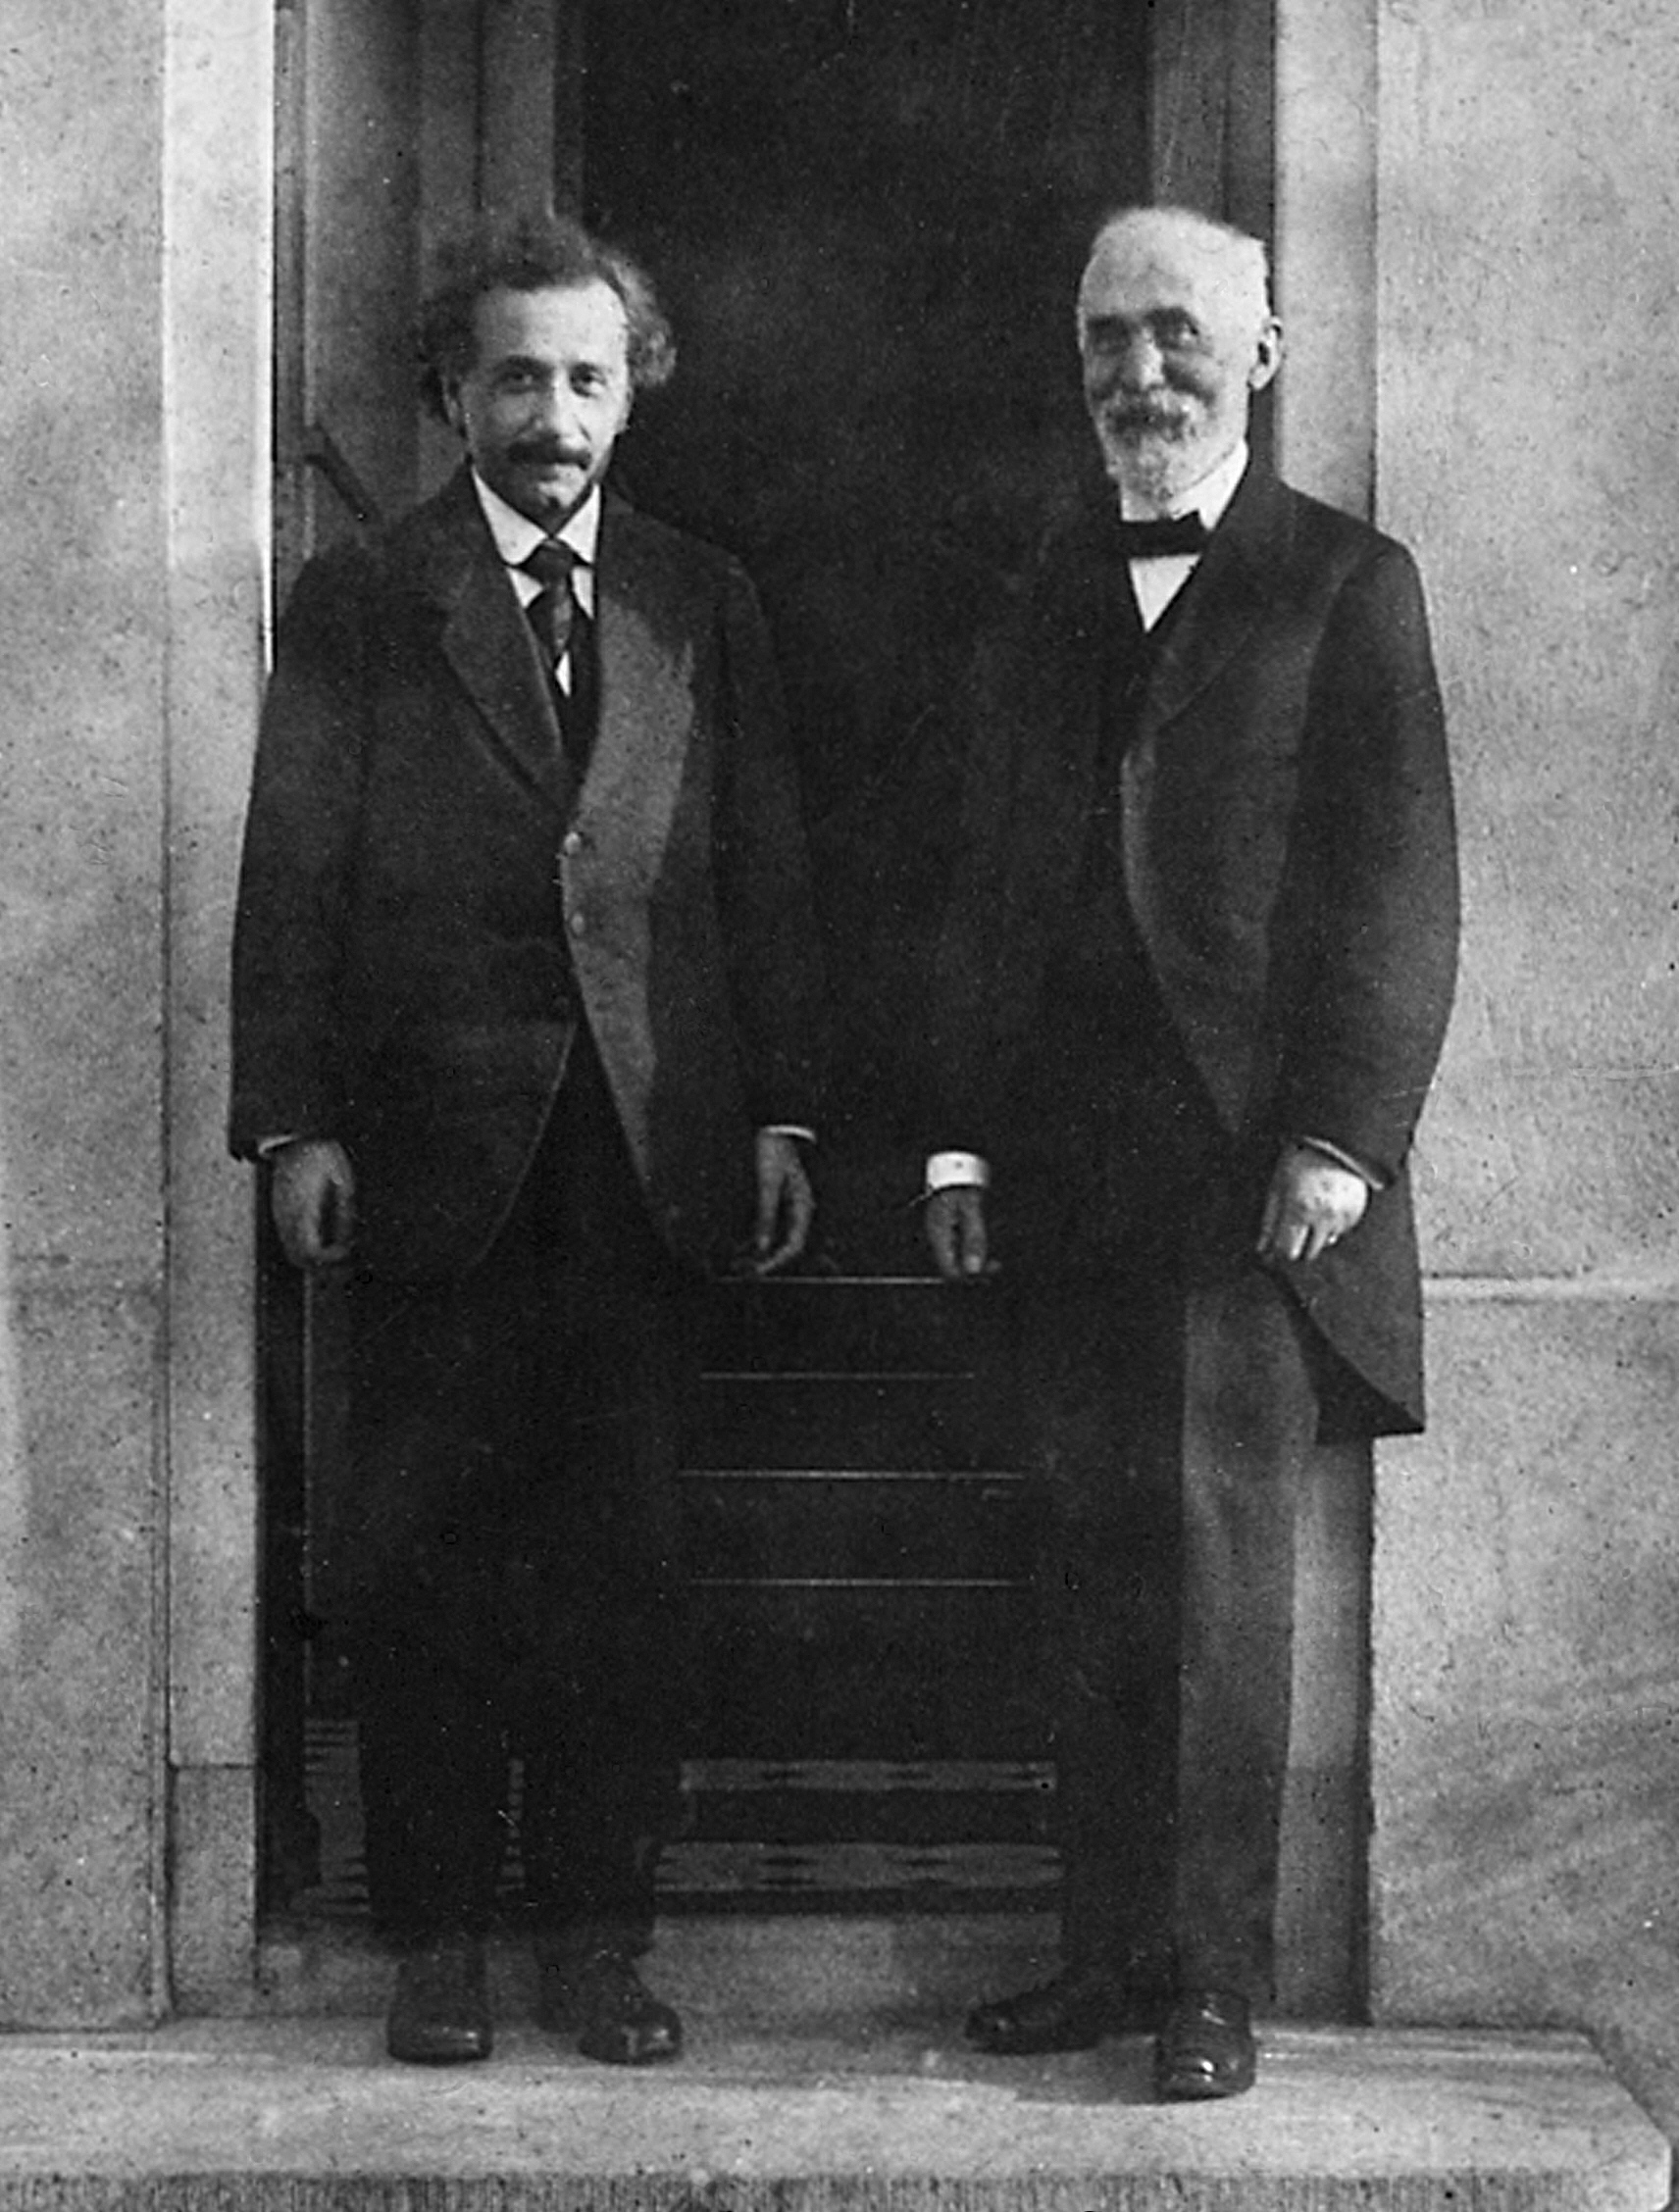
\includegraphics[width=6cm]{image/18-1-2.jpg}
\caption{\rm Einstein与Lorentz}
\end{wrapfigure}

历史上虽然电子作为粒子的发现是1897年\emph{汤姆孙}({\rm J. J. Thomson})的工作.\,但是早在半个世纪前人们就开始逐渐相信物质由两种带电粒子构成并在导电时可以移动的模型了.\,人们用这样的模型去想象输运现象,\,电磁感应,\,热电耦合等现象并取得了丰硕的成果,\,经典电磁学早在1860年代便在\emph{麦克斯韦}({\rm J. C. Maxwell})的工作下达到顶点进入尾声.\,剩下来的几十年时间历史让位给了\emph{洛伦兹}({\rm H. A. Lorentz}),\,洛伦兹对电磁学的贡献是深远的.\,他承前人之大成,\,讨论电磁场与电磁介质的相互作用,\,讨论电磁学原理与古老的伽利略式相对性原理的结合;\,又开近代物理之先河,\,电子论自然地导向了量子理论,\,而电磁学又自然地促成了狭义相对论的诞生.\,事实上,\,早年间狭义相对论在学界被介绍时便是以洛伦兹和爱因斯坦这一对忘年交命名的洛伦兹-爱因斯坦理论.

电子,\,这样一个基本粒子可以说是妇孺皆知的概念,\,它带一个单位的负电荷,\,其基本参数为:
\[e=1.602176634\times 10^{-19}{\rm C}\qquad m_e=9.10938356\times 10^{-34}{\rm kg}\]

然而出于各种原因,\,在经典电子论中的电子却又是一个陌生的概念.\,根据洛伦兹的经典电子论精神,\,重的原子实被认为静止,\,轻的束缚电子被认为在外场中可以运动,\,且主要受电场的影响\footnote{根据洛伦兹力公式$\bs{F}=q(\bs{E}+\bs{v}\times\bs{B})$,\,而电磁场中$E=cB$,\,故$v\ll c$时磁场力可以忽略.}.\,电子在外电场中相对原子实的位移造成了电偶极矩.\,出于好的近似,\,将电子视作被绑在连接中心的弹簧的另一端的质点.\,质量为$m$不再被认为与基本粒子的质量一致,\,事实上这个质量的本质实际上是虚无的,\,因为当考虑到原子与电磁场相互作用的严格理论时图像将完全是量子的而超出了此处可以讨论的范围,\,这样的一个为了解释现象去构造的模型就叫\emph{唯象模型}(phenomenological model).\,但是其电荷量还是$-e$,\,弹簧劲度系数为$k$.\,这样子我们就可以写出电子在外电场中的动力学方程:
\[m\bs{\ddot{r}}+k\bs{r}=-e\bs{E}\]

但是我们还忽略了一点,\,加速运动的电荷会产生辐射,\,也会因为辐射而带走能量和动量,\,这就被视作介质对电磁波吸收,\,散射的根本原因.\,也同样为了唯象地描述它,\,我们认为电子是受到了一个阻尼力$\bs{f}=-\gamma \bs{v}$.\,这样以上方程就被修改为:
\[m\bs{\ddot{r}}+\gamma \bs{\dot{r}}+k\bs{r}=-e\bs{E}\]

命$\omega_0=\sqrt{k/m}$代表\emph{共振频率}(resonance frequency)或待会就会说明的\emph{吸收频率}(absorption frequency).\,再命入射电磁波为频率$\omega$的光,\,按光学符号约定$\bs{E}=\bs{E}_0\ue^{-\ui\omega t}$,\,那么很容易解出受迫振动解$\bs{r}=\bs{r}_0\ue^{-\ui\omega t}$,\,振幅为:
\[\bs{r}_0=\frac{-e\bs{E}_0/m}{\omega_0^2-\omega^2-\ui\gamma\omega/m}\]

我们现在就能算出动态的分子极化率来,\,它被定义为分子中$Z$个价电子产生的偶极矩$\bs{p}=-Ze\bs{r}_0$与外电场$\bs{E}_0$的比值,\,可以发现它也是个复数,\,依赖于外光场的频率:
\[\alpha(\omega)=\frac{Ze^2/m}{\omega_0^2-\omega^2-\ui\gamma\omega/m}\]

我们知道,\,对于具体介质的极化总是与各个单元的极化有关.\,我们在此讨论稀薄的无固有偶极矩的气体在外电磁波中的极化\footnote{如果是液体或固体,\,一方面由于不同的偶极子间的相互影响不可忽略导致公式需要修正,\,也因为极化方式还有取向极化等所以需要修正,\,但全都只影响定量结果,\,定性的图像仍然是适用的.},\,此时不难想到介质的介电常数应该直接依赖于分子极化率,\,事实上,\,极化强度为:
\[\bs{P}=\chi\varepsilon_0\bs{E}=(\varepsilon_r-1)\varepsilon_0\bs{E}=n\bs{p}\]


从而得到复电容率的值:
\[\varepsilon'=\varepsilon_0+\frac{nZe^2/m}{\omega_0^2-\omega^2-\ui\gamma\omega/m}\]

\begin{wrapfigure}[15]{o}[0pt]{6cm}
\centering
\vspace{-15pt}
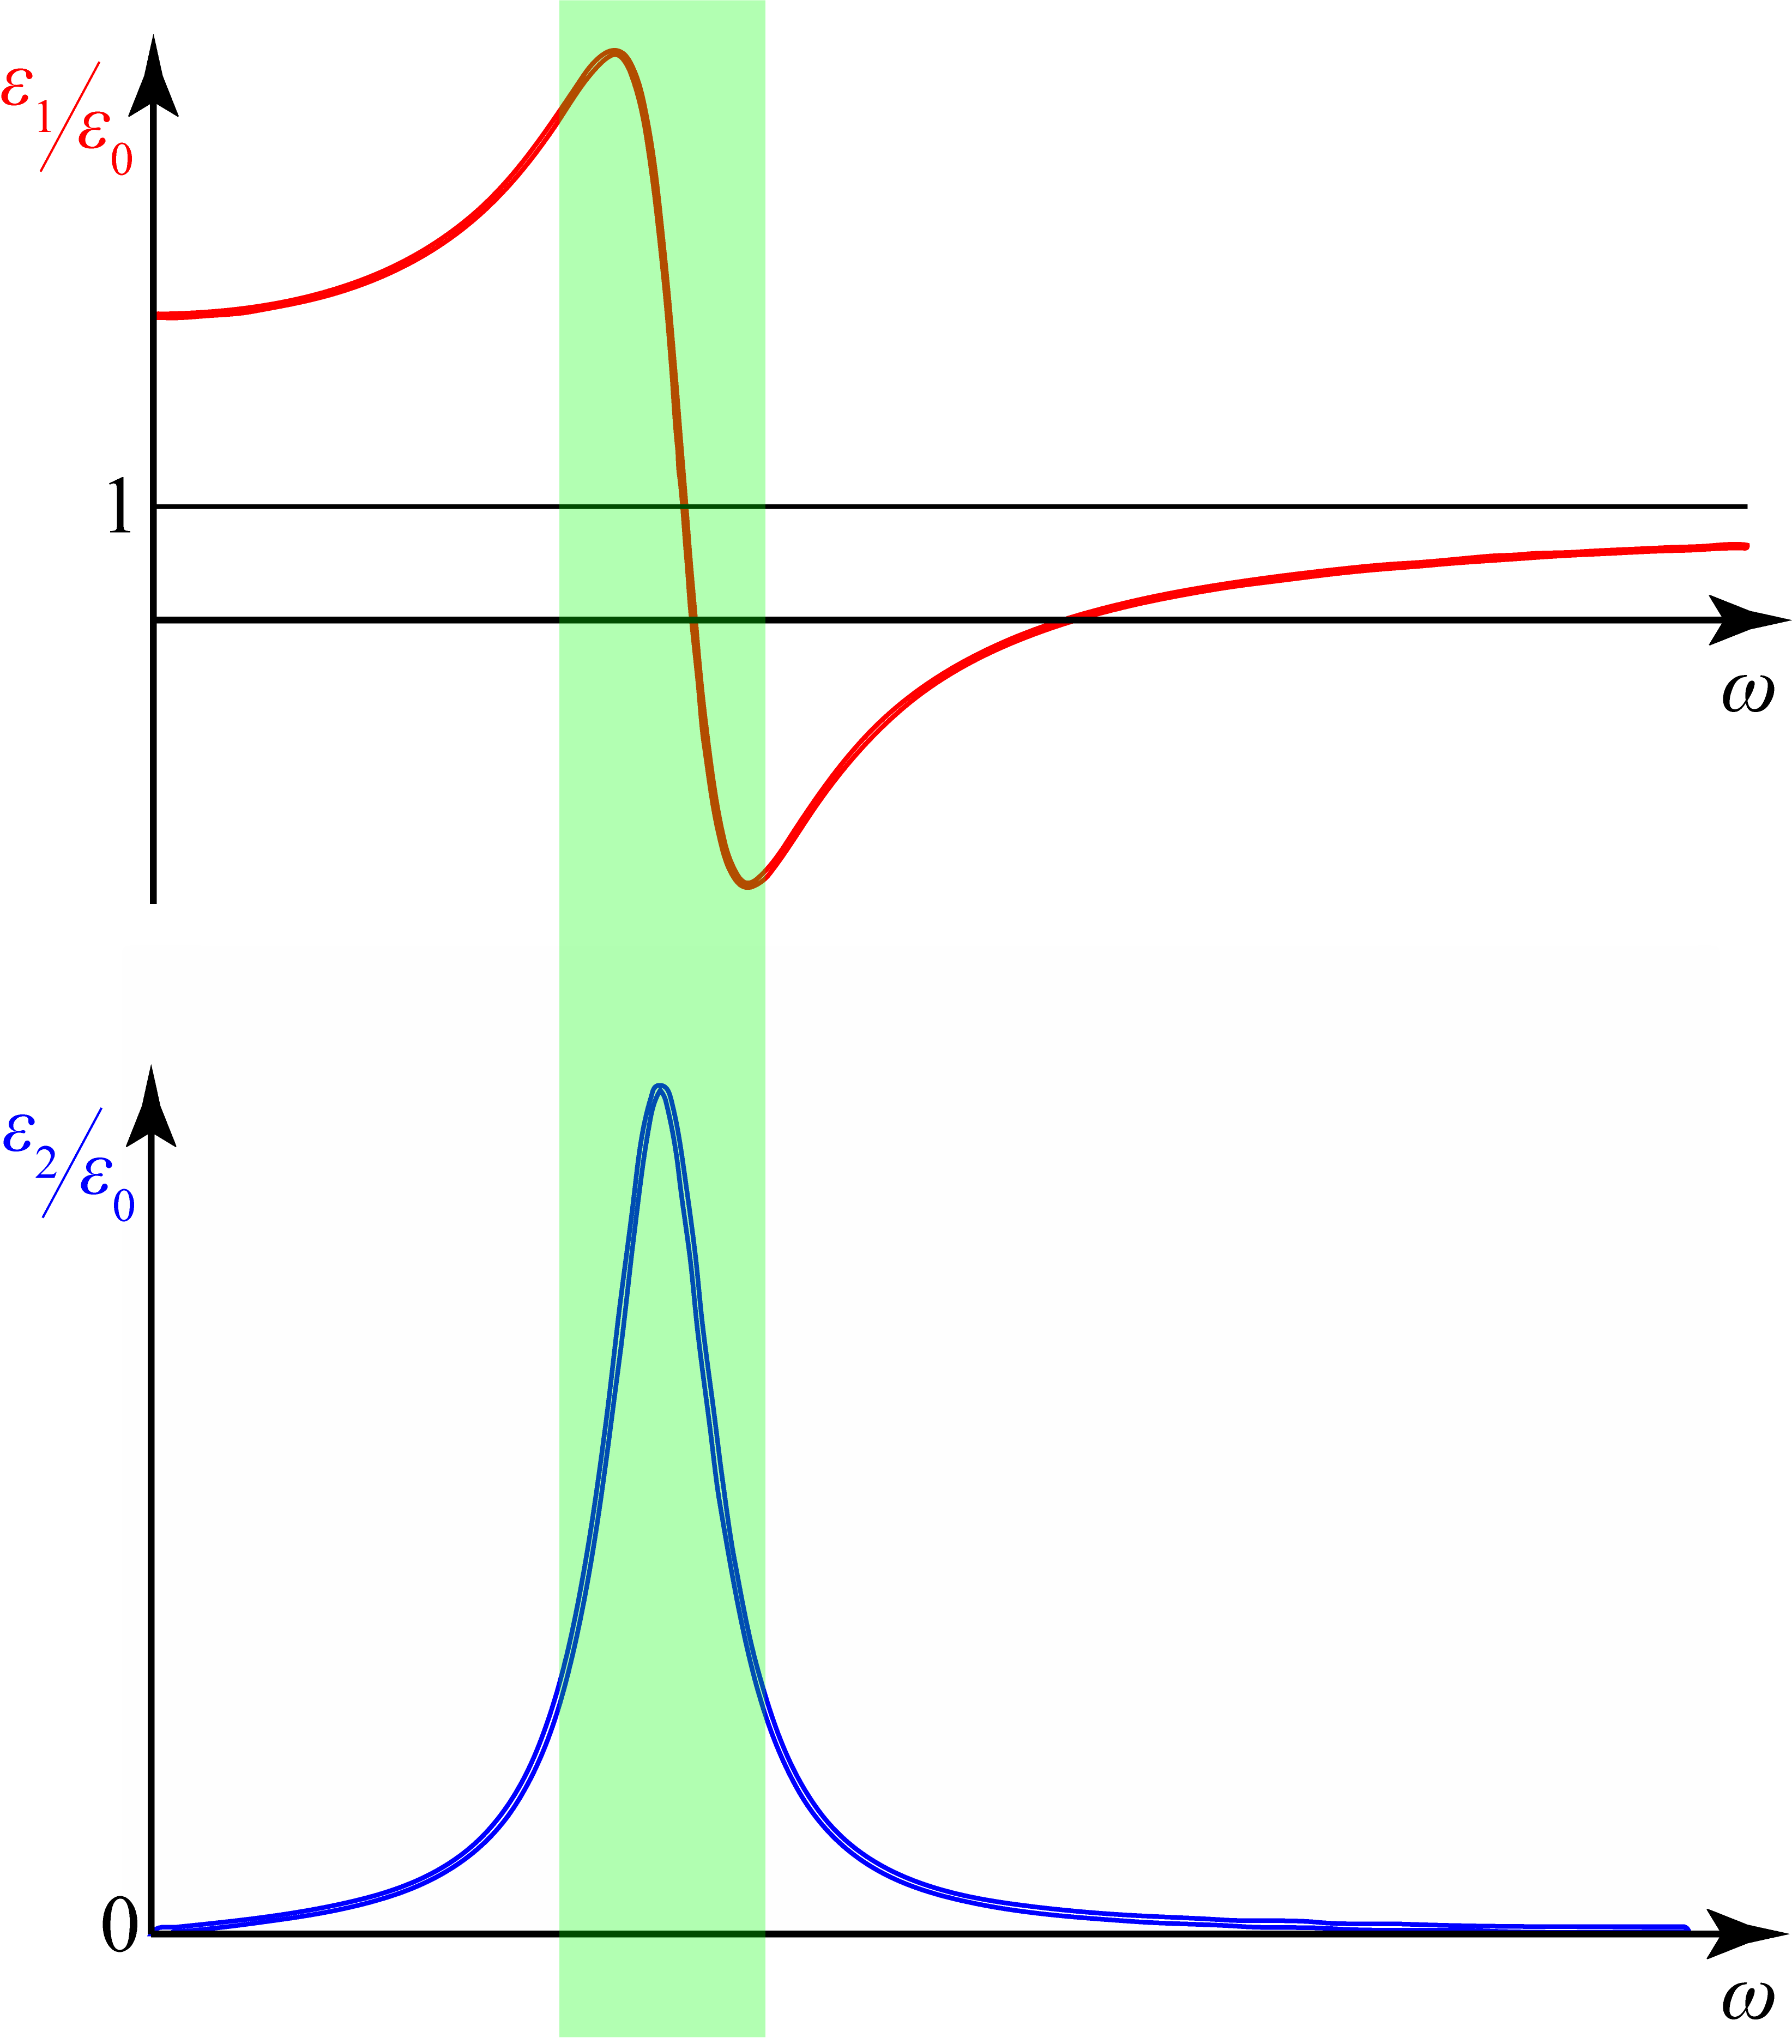
\includegraphics[width=6cm]{image/18-1-1.png}
\caption{复电容率与频率的关系}
\end{wrapfigure}
通常,\,把$nZe^2/\varepsilon_0 m$称作\emph{等离子体频率}(plasma frequency)的平方$\omega_p^2$.\,那么上式也作:
\[\varepsilon'=\varepsilon_0+\frac{\omega_p^2}{\omega_0^2-\omega^2-\ui\gamma\omega/m}\varepsilon_0\]

出现虚部其实就意味着损耗,\,在振动的过程中电场在持续不断地对振子输入能量而导致了电磁波的衰减.\,只不过这里的损耗并不是导电行为导致的.\,写出复电容率的实部和虚部$\varepsilon'=\varepsilon_1+\ui\varepsilon_2$:
\[\varepsilon_1=\varepsilon_0\cdot\left[1+\frac{\omega_p^2(\omega_0^2-\omega^2)}{(\omega_0^2-\omega^2)^2+(\gamma\omega/m)^2}\right]\]
\[\varepsilon_2=\varepsilon_0\cdot\frac{\gamma\omega_p^2\omega/m}{(\omega_0^2-\omega^2)^2+(\gamma\omega/m)^2}\]

两个函数看上去复杂,\,其实都属于近似的\emph{洛伦兹型函数}(lorentzian function).\,图像如右图所示.\,在绿色带状区域这个函数有着较大的转折.\,这发生在$\omega\approx \omega_0$处.\,若做近似,\,认为反应损耗的$\gamma$较小.\,则命$\omega^2-\omega_0^2=x$,\,$\gamma\omega_0/m=a$,\,那么上式在带状区域附近近似为标准的洛伦兹型:
\[\varepsilon_1/\varepsilon_0=1-\omega_p^2\cdot \frac{x}{x^2+a^2}\]
\[\varepsilon_2/\varepsilon_0=\omega_p^2\cdot\frac{a}{x^2+a^2}\]

电容率的实部在带状区域由区域外的缓慢增加转为剧烈减少,\,而恰好在这样一个区域,\,电容率的虚部突然变得很大.\,我们习惯上用虚部这种洛伦兹函数增加到最大值的一半的两个点之间的间距作为特征的\emph{半高峰宽}(full width at half maximum,\,FWHM).\,对于洛伦兹型,\,其值恰为$x=\pm a$之间的间距$2a$,\,但是注意到要转化为$\omega$对应的间距,\,它恰好为:
\[\Gamma=\frac{\gamma}{m}\]

我们可以从这个模型中清楚地看到两个物理现象:\,\emph{色散}(dispersion)与\emph{吸收}(absorption).\,前者就是说折射率依赖于波长,\,这和复电容率的实部依赖于频率只是说法不同本质一样.\,而复电容率的虚部,\,根据之前的讨论,\,也就代表吸收.\,我们发现在入射光的频率近似为谐振子的固有频率$\omega_0$时,\,对应经典力学中发生共振的区域附近,\,色散和吸收都变得很显著.\,我们知道,\,经典电子论给出的解释仅仅是一个唯象模型,\,所以相关的参数都要根据实验结果来确定.\,$\omega_0$可以根据发生强烈吸收与色散的波长来确定,\,而$\gamma/m$则根据吸收峰的半高峰宽$\Gamma$来确定,\,最后等离子体频率$\omega_p$则比较有趣,\,我们恰好可以根据零频率处的折射率$n_0$来确定它:
\[n_0^2=\varepsilon_1(0)/\varepsilon_0=1+\omega_p^2/\Gamma^2\]


那么实际情况是否这么简单呢?\,至少通过对右图的常温下水的色散的测量中我们发现,\,除了在可见光波段水几乎是透明的而具有大约$1.33$的折射率,\,在近红外(0.8-2.5${\rm \upmu m}$)与中红外(2.5-15${\rm \upmu m}$)波段的短波区定性上符合以上模型推导出来的结果.\,但是中红外到远红外(15-1000${\rm \upmu m}$)则明显偏离以上结果.
\begin{figure}[H]
\centering
\begin{minipage}{0.53\textwidth}
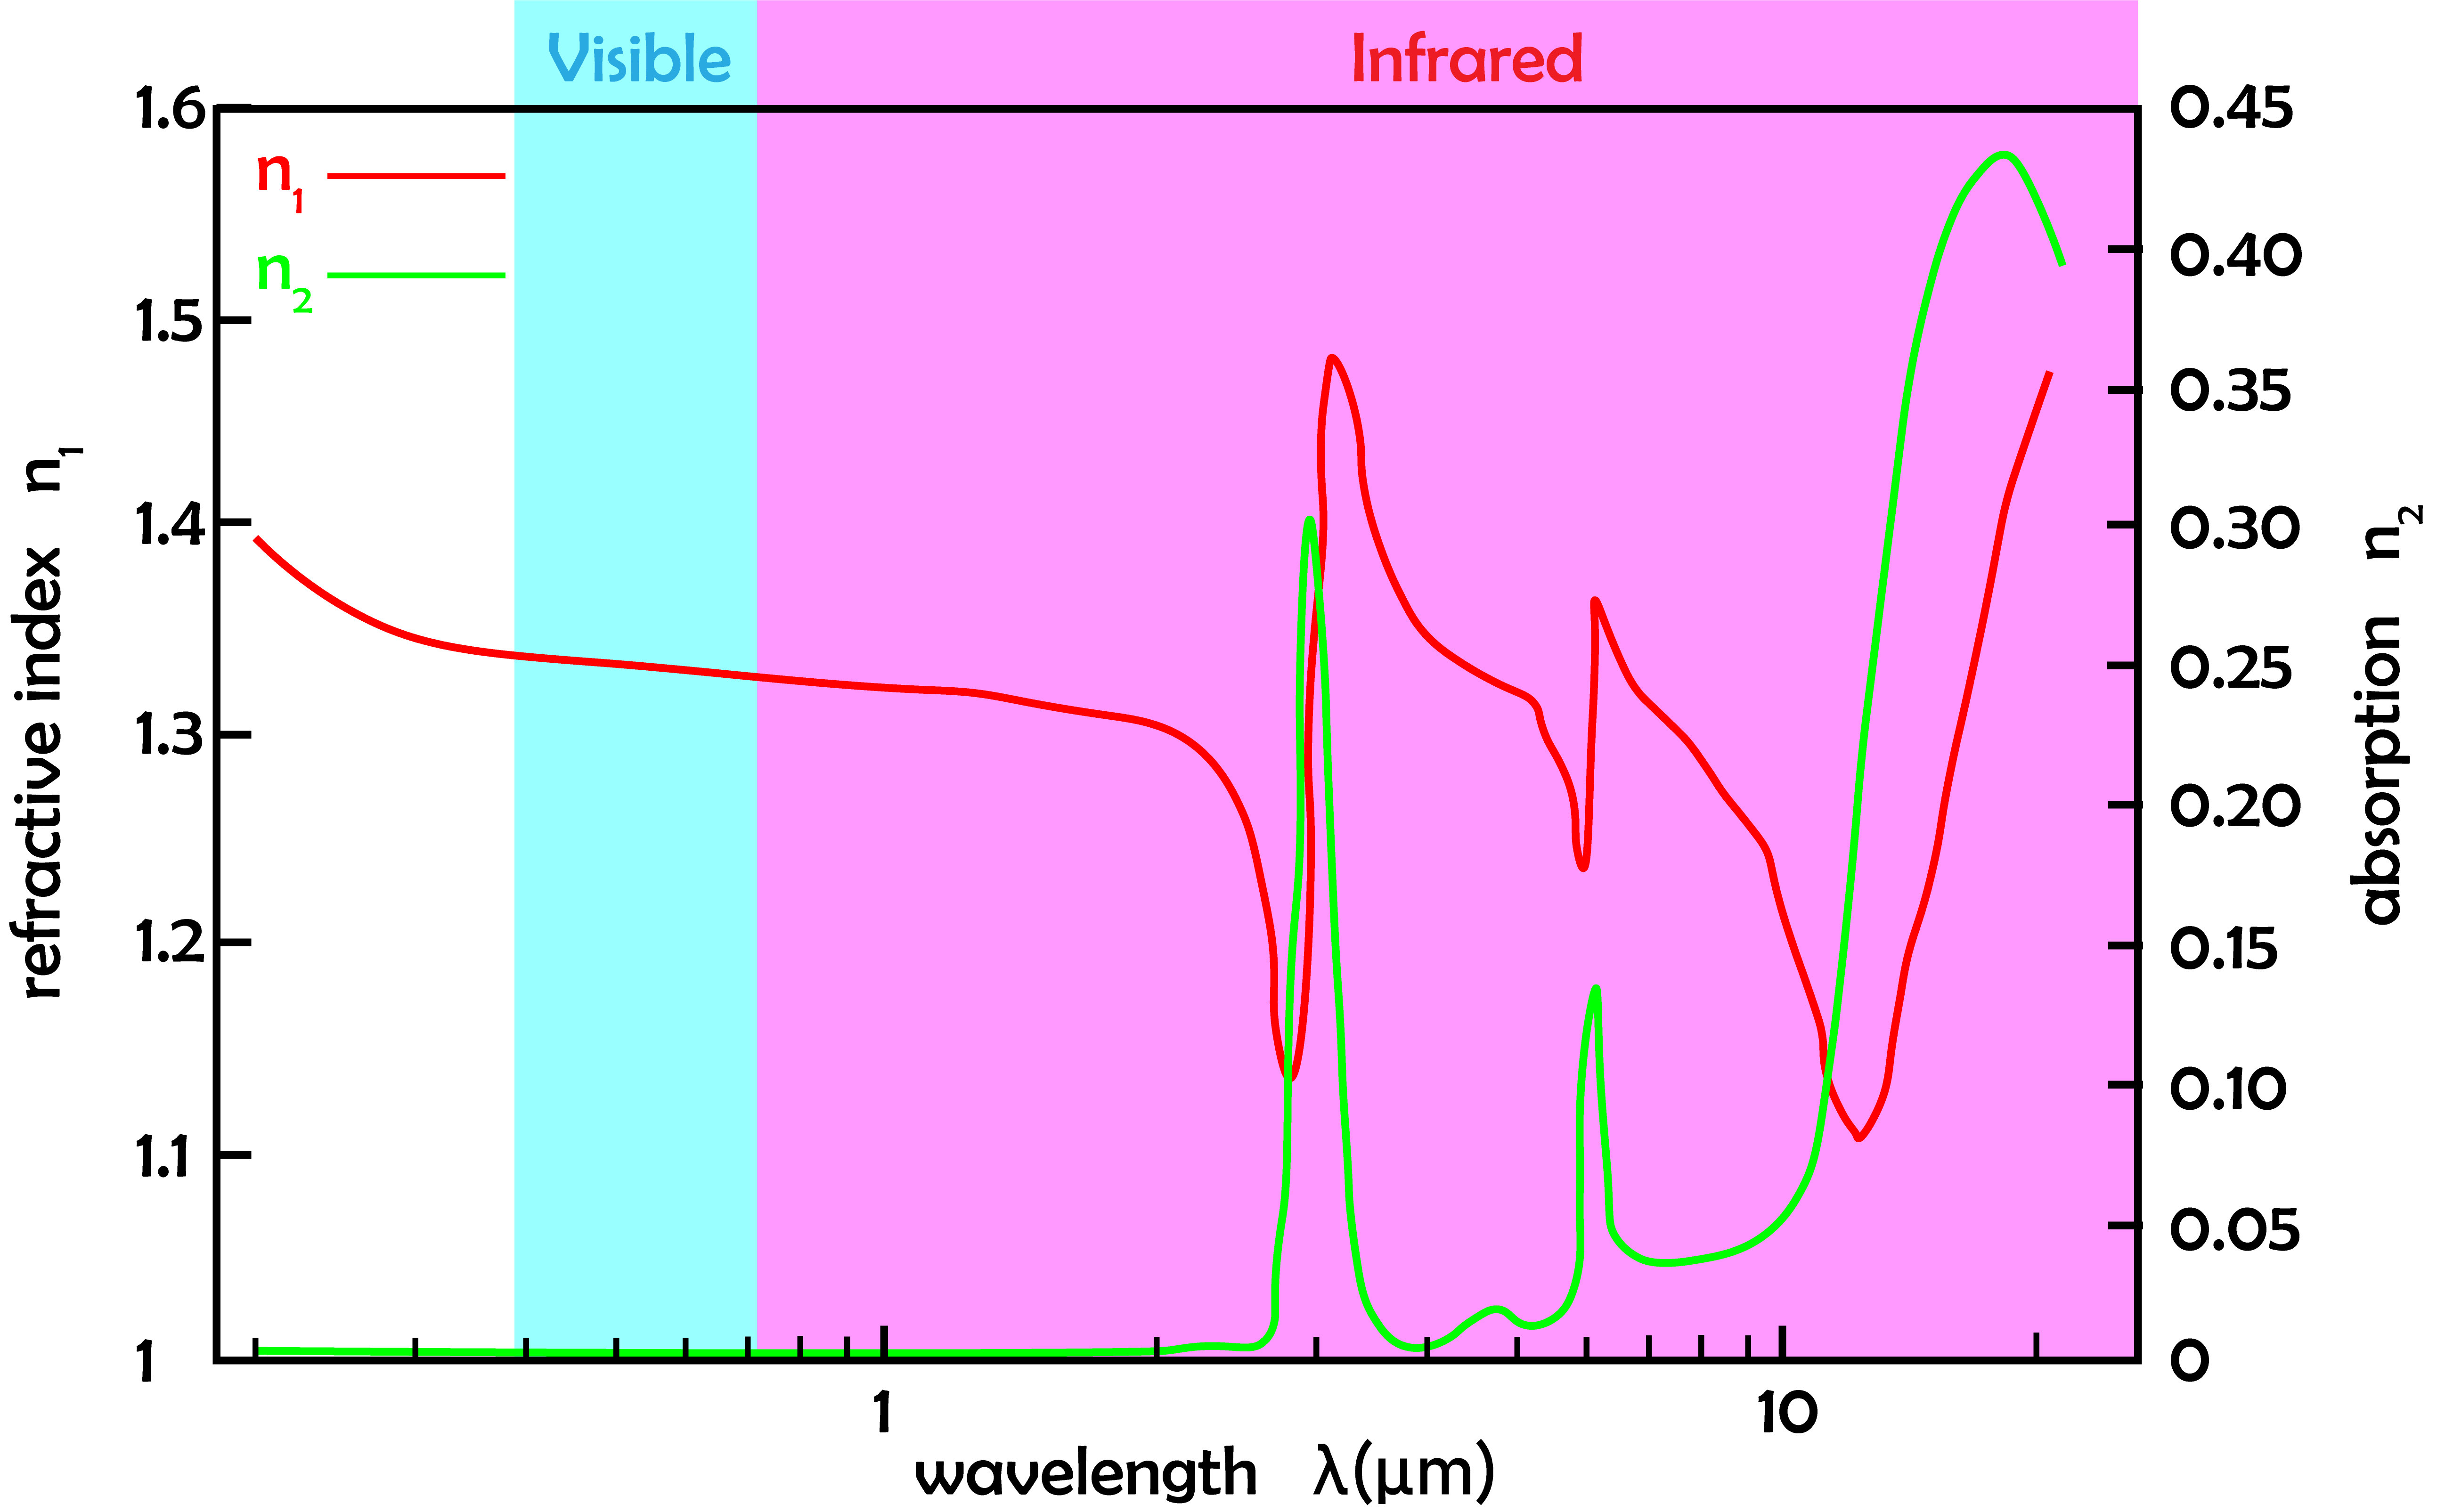
\includegraphics[width=\textwidth]{image/18-1-3.png}
\caption{水的可见-红外色散曲线}
\end{minipage}
\qquad
\begin{minipage}{0.38\textwidth}
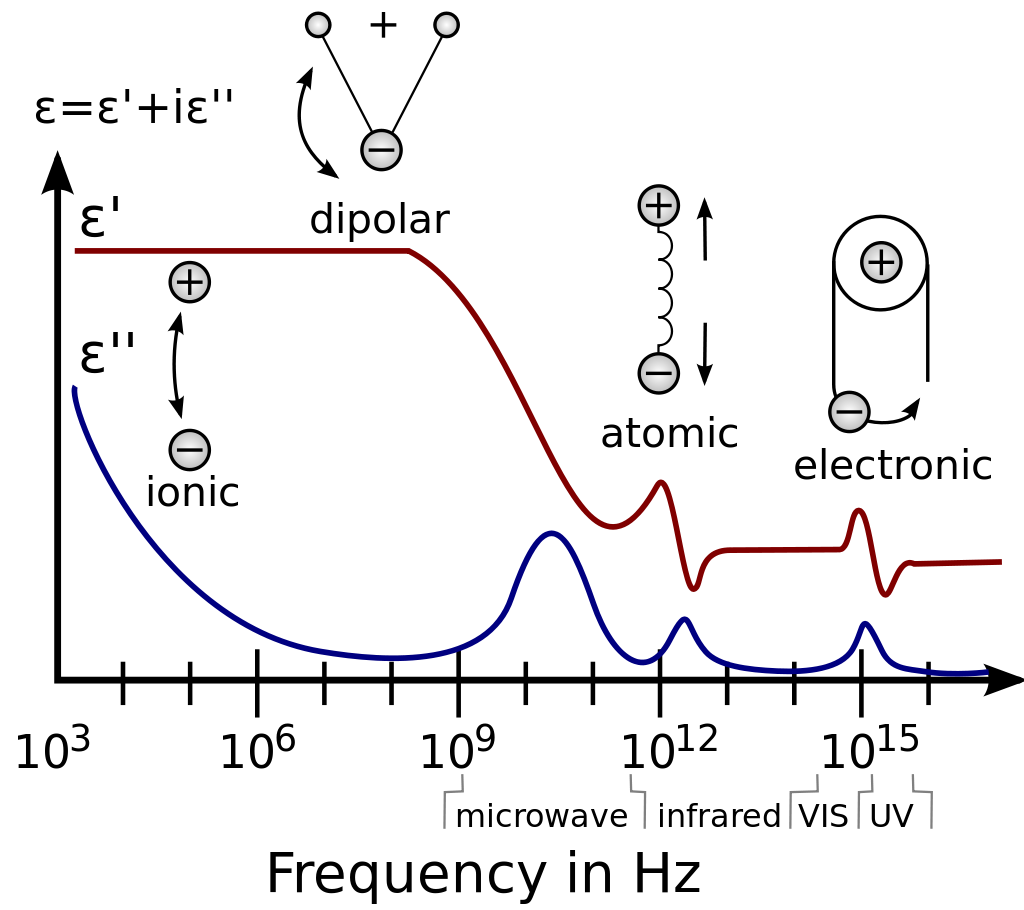
\includegraphics[width=\textwidth]{image/18-1-4.png}
\caption{光与原子作用类型}
\end{minipage}
\end{figure}

事实上,\,在不同的波段,\,适用于不同的光与物质相互作用的基本模型.\,微波波段光波长足够长使得晶体的正负离子做大范围的整体相对运动\footnote{十分类似于热运动的那种形式,\,区别在于这是外场诱导的有规律的振动,\,而且正负电荷位移一定反相,\,对应热振动的特定光学支.},\,就是晶格振动.\,红外则开始使得分子振动,\,包括转动和振动等不同形式.\,再往下的可见波段才是电子共振,\,也包括原子间的能带共振和原子内的能级共振.\,最后在紫外波段,\,电子甚至能直接被电离,\,这就造成了光与物质相互作用问题的复杂性.

但无论哪种相互作用的机制,\,我们上述推导得到的描述有着特定共振频率的色散与吸收的最终公式是十分普适的.\,它只有三个待定的参数:\,共振频率$\omega_0$,\,半高峰宽$\Gamma$和反应共振强度的等离子体频率$\omega_p$.\,我们接下来要做的,\,是把不同振子,\,不同吸收效应带来的结果进行求和:
\[\varepsilon_1/\varepsilon_0=1+\omega_p^2\cdot\sum_i\frac{c_i(\omega_i^2-\omega^2)}{(\omega_i^2-\omega^2)^2+\Gamma_i^2\omega^2}\]
\[\varepsilon_2/\varepsilon_0=\omega_p^2\cdot\sum_i\frac{c_i\Gamma_i\omega}{(\omega_i^2-\omega^2)^2+\Gamma_i^2\omega^2}\]

其中$\omega_p$仍然统计各个吸收峰的总强度,\,而$c_i$系数的和必须为1则统计各个吸收峰的相对强度.\,我们最后计算远离吸收带处的折射率值.\,忽略各个$\Gamma_i$后得到:
\[n^2=1+\omega_p^2\cdot\sum_i\frac{c_i}{\omega_i^2-\omega^2}\]

上式就是著名的\emph{塞尔迈耶尔方程}(Selmeyer'
s equation),\,如果用波长表示则为:
\[n^2=1+\sum_i a_i\cdot\frac{\lambda^2}{\lambda^2-\lambda_i^2}\quad,\quad a_i=\frac{c_i\omega_p^2\lambda_i^2}{4\pi^2c^2}\]

上式依然可以做近似,\,把共振的各个波长$\lambda_i$从小到大按$i$来排列.\,不妨设$\lambda_i\ll\lambda_{i+1}$,\,而$\lambda$恰好接近$\lambda_i$,\,那么忽略所有$\lambda_{i+1}$及之后对应的小量项并将$\lambda_{i-1}$及之前的项直接近似为$a_i$:
\[n^2\approx 1+a_1+a_2+\cdots+a_{i-1}+\frac{a_i\lambda^2}{\lambda^2-\lambda_i^2}\]
\[= 1+a_1+a_2+\cdots+a_{i-1}+a_i+\frac{a_i\lambda_i^2}{\lambda^2-\lambda_i^2}\]
\[\approx 1+a_1+a_2+\cdots+a_{i-1}+a_i+\frac{a_i\lambda_i^2}{\lambda^2}\]
\[=A_0+\frac{B_0}{\lambda^2}\]

而进一步近似得到:
\[\sqrt{A_0+\frac{B_0}{\lambda^2}}=\sqrt{A_0}\left(1+\frac{B_0}{A_0\lambda^2}\right)^{1/2}=\sqrt{A_0}\left(1+\frac{B_0}{2A_0\lambda^2}-\frac{B_0^2}{8A_0^2 \lambda^4}+\cdots\right)\]

一般就总结为如下\emph{柯西色散公式}(Cauchy dispersion formula):
\[n(\lambda)=A+\frac{B}{\lambda^2}\]

有时为了精度原因再加上四阶项$+C/\lambda^4$.\,而从推导过程中我们发现系数之间的联系:
\[A=\sqrt{1+\sum_1^i a_i}\quad ,\quad B=\frac{a_i\lambda_i^2}{2A}\]


%\section{色散,\,散射与吸收}

%\section{群速与展宽}

%\section{光量子}

